%%%%%%%%%%%%%%%%%%%%%%%%%%%%%%%%%%%%%%%%%%%%%%%%%%%%%%%%%%%%%%%%%%%%%%%%%%%%%%%
%
% Vignette  "How to generate new distributions in packages distr, distrEx"
%
%
%%%%%%%%%%%%%%%%%%%%%%%%%%%%%%%%%%%%%%%%%%%%%%%%%%%%%%%%%%%%%%%%%%%%%%%%%%%%%%%
%
%\VignetteIndexEntry{newDistributions}
%\VignetteDepends{startupmsg}
%\VignetteKeywords{probability distribution,estimation}
%\VignettePackage{distr}                     
%
%
%
\documentclass[10pt]{article}
%
%use svn-multi to fill in revision information
%
\usepackage{svn-multi}
% Version control information:
\svnidlong
{$HeadURL: svn+ssh://ruckdeschel@svn.r-forge.r-project.org/svnroot/distr/pkg/distr/inst/doc/newDistributions.Rnw $}
{$LastChangedDate: 2009-03-24 11:49:33 +0100 (Di, 24 Mrz 2009) $}
{$LastChangedRevision: 439 $}
{$LastChangedBy: ruckdeschel $}
%\svnid{$Id: example_main.tex 146 2008-12-03 13:29:19Z martin $}
% Don't forget to set the svn property 'svn:keywords' to
% 'HeadURL LastChangedDate LastChangedRevision LastChangedBy' or
% 'Id' or both depending if you use \svnidlong and/or \svnid
%
\newcommand{\svnfooter}{Last Changed Rev: \svnkw{LastChangedRevision}}
\svnRegisterAuthor{ruckdeschel}{Peter Ruckdeschel}
\svnRegisterAuthor{stamats}{Matthias Kohl}
\svnRegisterAuthor{florian}{Florian Camphausen}
\svnRegisterAuthor{stabla}{Thomas Stabla}
\svnRegisterAuthor{anhuel}{Anja H{\"u}ller}
\svnRegisterAuthor{ifrin}{Eleonara Feist}
\svnRegisterAuthor{jdospina}{Juan David Ospina}
\svnRegisterAuthor{kowzar}{Kouros Owzar}
%
\usepackage{geometry}
%
\usepackage{color}
\definecolor{darkblue}{rgb}{0.0,0.0,0.75}
\definecolor{distrCol}{rgb}{0.0,0.4,0.4}
%
\usepackage{ifpdf}
%
\usepackage{amssymb}
\usepackage[%
baseurl={r-forge.r-project.org},%
pdftitle={How to generate new distributions in packages distr, distrEx},%
pdfauthor={Peter Ruckdeschel, Matthias Kohl},%
pdfsubject={distr},%
pdfkeywords={probability distribution,simulation,estimation},%
pagebackref,bookmarks,colorlinks,linkcolor=darkblue,citecolor=darkblue,%
pagecolor=darkblue,raiselinks,plainpages,pdftex]{hyperref}
%
\markboth{\sl How to generate new distributions in packages ``{\tt distr}'', ``{\tt distrEx}''}%
{\sl How to generate new distributions in packages ``{\tt distr}'', ``{\tt distrEx}''}
%
% -------------------------------------------------------------------------------
\newcommand{\Reals}{\mathbb{R}}
\newcommand{\R}{\mathbb{R}}
\newcommand{\N}{\mathbb{N}}
%
% -------------------------------------------------------------------------------
\RequirePackage{listings}
\usepackage{Sweave}
% -------------------------------------------------------------------------------

% -------------------------------------------------------------------------------
%------------------------------------------------------------------------------%
%Preparations for Sweave and Listings
%------------------------------------------------------------------------------%
%
\RequirePackage{color}
\definecolor{Rcolor}{rgb}{0, 0.5, 0.5}
\definecolor{Rbcolor}{rgb}{0, 0.6, 0.6}
\definecolor{Rout}{rgb}{0.461, 0.039, 0.102}
\definecolor{Rcomment}{rgb}{0.101, 0.043, 0.432}
%------------------------------------------------------------------------------%
\lstdefinelanguage{Rd}[common]{TeX}%
  {moretexcs={acronym,alias,arguments,author,bold,cite,%
          code,command,concept,cr,deqn,describe,%
          description,details,dfn,docType,dots,%
          dontrun,dontshow,donttest,dQuote,%
          email,emph,enc,encoding,enumerate,env,eqn,%
          examples,file,format,item,itemize,kbd,keyword,%
          keyword,ldots,link,linkS4class,method,name,note,%
          option,pkg,preformatted,R,references,S3method,%
          S4method,samp,section,seealso,source,sp,special,%
          sQuote,strong,synopsis,tab,tabular,testonly,%
          title,url,usage,value,var},
   sensitive=true,%
   morecomment=[l]\%% 2008 Peter Ruckdeschel
}[keywords,comments]%%
%------------------------------------------------------------------------------%
\lstdefinestyle{Rstyle}{fancyvrb=true,escapechar=`,language=R,%
                        basicstyle={\color{Rcolor}\small},%
                        keywordstyle={\bf\color{Rcolor}},%
                        commentstyle={\color{Rcomment}\ttfamily\itshape},%
                        literate={<-}{{$\leftarrow$}}2{<<-}{{$\twoheadleftarrow$}}2,%
                        alsoother={$},%
                        alsoletter={.<-},%
                        otherkeywords={!,!=,~,$,*,\&,\%/\%,\%*\%,\%\%,<-,<<-,/}}%
\lstdefinestyle{Rdstyle}{fancyvrb=true,language=Rd,keywordstyle={\bf},%
                         basicstyle={\color{black}\footnotesize},%
                         commentstyle={\ttfamily\itshape},%
                         alsolanguage=R}%
%------------------------------------------------------------------------------%
\global\def\Rlstset{\lstset{style=Rstyle}}%
\global\def\Rdlstset{\lstset{style=Rdstyle}}%
\Rlstset
%------------------------------------------------------------------------------%
\DefineVerbatimEnvironment{Sinput}{Verbatim}%
  {formatcom=\color{Rcolor}\lstset{fancyvrb=true,escapechar='}}
\DefineVerbatimEnvironment{Soutput}{Verbatim}%
  {formatcom=\color{Rout}\small\lstset{fancyvrb=false}}
\DefineVerbatimEnvironment{Scode}{Verbatim}%
  {fontshape=sl,formatcom=\color{Rcolor}\lstset{fancyvrb=true}}
%------------------------------------------------------------------------------%
\ifthenelse{\boolean{Sweave@gin}}{\setkeys{Gin}{width=0.8\textwidth}}{}%
%------------------------------------------------------------------------------%
\let\code\lstinline
\def\Code#1{{\tt\color{Rcolor} #1}}
\def\file#1{{\tt #1}}
\def\pkg#1{{\tt "#1"}}
\newcommand{\pkgversion}{{\tt 2.1.1}}
%------------------------------------------------------------------------------%
% --------------------------
% Registration of package SweaveListingUtils
% --------------------------
\lstset{morekeywords={[2]changeKeywordstyles,copySourceFromRForge,getSweaveListingOption,lstinputSourceFromRForge,lstset,%
lstsetLanguage,lstsetR,lstsetRd,readPkgVersion,readSourceFromRForge,%
setToBeDefinedPkgs,SweaveListingMASK,SweaveListingoptions,SweaveListingOptions,SweaveListingPreparations,%
taglist%
},%
keywordstyle={[2]{\bf}}%
}
%
%

% --------------------------
% Registration of package startupmsg
% --------------------------
\lstset{morekeywords={[3]buildStartupMessage,infoShow,mySMHandler,mystartupMessage,NEWS,%
onlytypeStartupMessages,pointertoNEWS,readURLInformation,readVersionInformation,startupEndline,%
startupMessage,StartupMessage,startupPackage,startupType,suppressStartupMessages%
},%
keywordstyle={[3]{\bf}}%
}
%
%

% --------------------------
% Registration of package tools
% --------------------------
\lstset{morekeywords={[4]Adobe_glyphs,buildVignettes,charset_to_Unicode,checkDocFiles,checkDocStyle,%
checkFF,checkMD5sums,checkNEWS,checkRd,checkReplaceFuns,%
checkS3methods,checkTnF,checkVignettes,codoc,codocClasses,%
codocData,delimMatch,dependsOnPkgs,encoded_text_to_latex,file_path_as_absolute,%
file_path_sans_ext,findHTMLlinks,getDepList,installFoundDepends,list_files_with_exts,%
list_files_with_type,md5sum,package.dependencies,parse_Rd,pkgDepends,%
pkgVignettes,Rd_db,Rd_parse,Rd2ex,Rd2HTML,%
Rd2latex,Rd2txt,Rdiff,Rdindex,read.00Index,%
readNEWS,showNonASCII,testInstalledBasic,testInstalledPackage,testInstalledPackages,%
texi2dvi,vignetteDepends,write_PACKAGES,xgettext,xgettext2pot,%
xngettext%
},%
keywordstyle={[4]{\bf}}%
}
%
%

% --------------------------
% Registration of package stats
% --------------------------
\lstset{morekeywords={[5]acf,acf2AR,add.scope,addmargins,aggregate.data.frame,%
aggregate.default,aggregate.ts,AIC,anova.glm,anova.glmlist,%
anova.lm,anova.lmlist,anova.mlm,anovalist.lm,ansari.test,%
ar,ar.burg,ar.mle,ar.ols,ar.yw,%
arima,arima.sim,arima0,arima0.diag,ARMAacf,%
ARMAtoMA,as.dendrogram,as.dist,as.formula,as.hclust,%
as.stepfun,as.ts,asOneSidedFormula,bandwidth.kernel,bartlett.test,%
binom.test,biplot,Box.test,bw.bcv,bw.nrd,%
bw.nrd0,bw.SJ,bw.ucv,cancor,case.names,%
ccf,chisq.test,clearNames,cmdscale,complete.cases,%
confint,confint.default,constrOptim,contr.helmert,contr.poly,%
contr.SAS,contr.sum,contr.treatment,contrasts<-,cooks.distance,%
cophenetic,cor.test,cov.wt,cov2cor,cpgram,%
cutree,decompose,delete.response,dendrapply,density.default,%
deriv.default,deriv.formula,deriv3,deriv3.default,deriv3.formula,%
df.kernel,df.residual,dfbeta,diff.ts,diffinv,%
dist,dmultinom,drop.scope,drop.terms,dummy.coef,%
ecdf,eff.aovlist,embed,estVar,expand.model.frame,%
factanal,factor.scope,filter,fisher.test,fitted.values,%
fligner.test,friedman.test,get_all_vars,getInitial,glm.control,%
glm.fit,glm.fit.null,hatvalues,hatvalues.lm,hclust,%
heatmap,HoltWinters,influence.measures,integrate,interaction.plot,%
inverse.gaussian,is.empty.model,is.leaf,is.mts,is.stepfun,%
is.ts,is.tskernel,isoreg,KalmanForecast,KalmanLike,%
KalmanRun,KalmanSmooth,kernapply,kernel,kmeans,%
knots,kruskal.test,ks.test,ksmooth,lag,%
lag.plot,line,lines.ts,lm.fit,lm.fit.null,%
lm.influence,lm.wfit,lm.wfit.null,loadings,loess,%
loess.control,loess.smooth,logLik,ls.diag,ls.print,%
make.link,makeARIMA,makepredictcall,manova,mantelhaen.test,%
mauchley.test,mauchly.test,mcnemar.test,median.default,medpolish,%
model.extract,model.frame,model.frame.aovlist,model.frame.default,model.frame.glm,%
model.frame.lm,model.matrix,model.matrix.default,model.matrix.lm,model.offset,%
model.response,model.tables,model.weights,monthplot,mood.test,%
na.action,na.contiguous,na.exclude,na.fail,na.omit,%
na.pass,napredict,naprint,naresid,nlminb,%
nls,nls.control,NLSstAsymptotic,NLSstClosestX,NLSstLfAsymptote,%
NLSstRtAsymptote,numericDeriv,oneway.test,order.dendrogram,p.adjust,%
p.adjust.methods,pacf,pairwise.prop.test,pairwise.t.test,pairwise.table,%
pairwise.wilcox.test,pbirthday,plclust,plot.density,plot.ecdf,%
plot.lm,plot.mlm,plot.spec,plot.spec.coherency,plot.spec.phase,%
plot.stepfun,plot.ts,plot.TukeyHSD,poisson.test,polym,%
power.anova.test,power.prop.test,power.t.test,PP.test,ppr,%
prcomp,predict.glm,predict.lm,predict.mlm,predict.poly,%
princomp,print.anova,print.coefmat,print.density,print.family,%
print.formula,print.ftable,print.glm,print.infl,print.integrate,%
print.lm,print.logLik,print.terms,print.ts,printCoefmat,%
promax,prop.test,prop.trend.test,qbirthday,qqnorm.default,%
quade.test,quantile.default,quasibinomial,quasipoisson,r2dtable,%
read.ftable,rect.hclust,reorder,reshape,reshapeLong,%
reshapeWide,residuals.default,residuals.glm,residuals.lm,rmultinom,%
rstandard.glm,rstandard.lm,rstudent.glm,rstudent.lm,runmed,%
scatter.smooth,screeplot,se.contrast,selfStart,setNames,%
shapiro.test,simulate,smooth,smooth.spline,smoothEnds,%
sortedXyData,spec.ar,spec.pgram,spec.taper,spectrum,%
splinefunH,SSasymp,SSasympOff,SSasympOrig,SSbiexp,%
SSD,SSfol,SSfpl,SSgompertz,SSlogis,%
SSmicmen,SSweibull,stat.anova,stepfun,stl,%
StructTS,summary.aov,summary.aovlist,summary.glm,summary.infl,%
summary.lm,summary.manova,summary.mlm,summary.stepfun,supsmu,%
t.test,termplot,terms.aovlist,terms.default,terms.formula,%
terms.terms,toeplitz,ts.intersect,ts.plot,ts.union,%
tsdiag,tsp<-,tsSmooth,TukeyHSD,TukeyHSD.aov,%
update.default,update.formula,var.test,variable.names,varimax,%
vcov,weighted.mean,weighted.residuals,wilcox.test,window<-,%
write.ftable,xtabs%
},%
keywordstyle={[5]{\bf}}%
}
%
%

% --------------------------
% Registration of package graphics
% --------------------------
\lstset{morekeywords={[6]assocplot,Axis,axis.Date,axis.POSIXct,axTicks,%
barplot.default,boxplot.default,boxplot.matrix,cdplot,clip,%
close.screen,co.intervals,contour.default,dotchart,erase.screen,%
filled.contour,fourfoldplot,grconvertX,grconvertY,hist.default,%
image.default,layout.show,lines.default,pairs.default,panel.smooth,%
pie,plot.default,plot.design,plot.new,plot.window,%
plot.xy,points.default,smoothScatter,spineplot,split.screen,%
strheight,stripchart,text.default,xspline%
},%
keywordstyle={[6]{\bf}}%
}
%
%

% --------------------------
% Registration of package grDevices
% --------------------------
\lstset{morekeywords={[7]as.graphicsAnnot,bitmap,blues9,bmp,boxplot.stats,%
bringToTop,check.options,CIDFont,cm.colors,col2rgb,%
colorConverter,colorRamp,colorRampPalette,colorspaces,contourLines,%
convertColor,densCols,dev.control,dev.copy,dev.copy2eps,%
dev.copy2pdf,dev.cur,dev.interactive,dev.list,dev.new,%
dev.next,dev.off,dev.prev,dev.print,dev.set,%
dev.size,devAskNewPage,deviceIsInteractive,embedFonts,extendrange,%
getGraphicsEvent,graphics.off,gray.colors,grey.colors,hcl,%
heat.colors,Hershey,jpeg,make.rgb,msgWindow,%
n2mfrow,nclass.FD,nclass.scott,nclass.Sturges,pdf,%
pdf.options,pdfFonts,png,postscriptFont,postscriptFonts,%
ps.options,recordGraphics,recordPlot,replayPlot,rgb2hsv,%
savePlot,setEPS,setPS,terrain.colors,tiff,%
topo.colors,trans3d,Type1Font,win.graph,win.metafile,%
win.print,windows,windows.options,windowsFont,windowsFonts,%
xfig,xy.coords,xyTable,xyz.coords%
},%
keywordstyle={[7]{\bf}}%
}
%
%

% --------------------------
% Registration of package utils
% --------------------------
\lstset{morekeywords={[8]alarm,argsAnywhere,as.person,as.personList,as.relistable,%
as.roman,assignInNamespace,available.packages,browseEnv,browseURL,%
browseVignettes,bug.report,capture.output,checkCRAN,choose.dir,%
choose.files,chooseCRANmirror,citation,citEntry,citFooter,%
citHeader,close.socket,combn,compareVersion,contrib.url,%
count.fields,CRAN.packages,data.entry,de.ncols,de.restore,%
de.setup,DLL.version,download.file,download.packages,dump.frames,%
file.edit,file_test,Filters,fixInNamespace,fixup.libraries.URLs,%
fixup.package.URLs,flush.console,formatOL,formatUL,getAnywhere,%
getClipboardFormats,getCRANmirrors,getFromNamespace,getIdentification,getS3method,%
getTxtProgressBar,getWindowsHandle,getWindowTitle,getWinProgressBar,glob2rx,%
head,head.matrix,help.request,help.search,help.start,%
history,index.search,install.packages,installed.packages,is.relistable,%
limitedLabels,link.html.help,loadhistory,loadRconsole,localeToCharset,%
ls.str,lsf.str,make.packages.html,make.search.html,make.socket,%
makeRweaveLatexCodeRunner,memory.limit,memory.size,mirror2html,modifyList,%
new.packages,normalizePath,object.size,old.packages,package.contents,%
package.skeleton,packageDescription,packageStatus,person,personList,%
promptData,promptPackage,rc.getOption,rc.options,rc.settings,%
rc.status,read.csv,read.csv2,read.delim,read.delim2,%
read.DIF,read.fortran,read.fwf,read.socket,read.table,%
readCitationFile,readClipboard,readRegistry,recover,relist,%
remove.packages,Rprof,Rprofmem,RShowDoc,RSiteSearch,%
rtags,Rtangle,RtangleSetup,RtangleWritedoc,RweaveChunkPrefix,%
RweaveEvalWithOpt,RweaveLatex,RweaveLatexFinish,RweaveLatexOptions,RweaveLatexSetup,%
RweaveLatexWritedoc,RweaveTryStop,savehistory,select.list,sessionInfo,%
setRepositories,setStatusBar,setTxtProgressBar,setWindowTitle,setWinProgressBar,%
shortPathName,stack,Stangle,str,strOptions,%
summaryRprof,Sweave,SweaveHooks,SweaveSyntaxLatex,SweaveSyntaxNoweb,%
SweaveSyntConv,tail,tail.matrix,timestamp,toBibtex,%
toLatex,txtProgressBar,type.convert,unstack,unzip,%
update.packages,update.packageStatus,upgrade,url.show,URLdecode,%
URLencode,View,vignette,win.version,winDialog,%
winDialogString,winMenuAdd,winMenuAddItem,winMenuDel,winMenuDelItem,%
winMenuItems,winMenuNames,winProgressBar,write.csv,write.csv2,%
write.socket,write.table,writeClipboard,wsbrowser,zip.file.extract,%
zip.unpack%
},%
keywordstyle={[8]{\bf}}%
}
%
%

% --------------------------
% Registration of package datasets
% --------------------------
\lstset{morekeywords={[9]ability.cov,airmiles,AirPassengers,airquality,anscombe,%
attenu,attitude,austres,beaver1,beaver2,%
BJsales,BJsales.lead,BOD,cars,ChickWeight,%
chickwts,co2,CO2,crimtab,discoveries,%
DNase,esoph,euro,euro.cross,eurodist,%
EuStockMarkets,faithful,fdeaths,Formaldehyde,freeny,%
freeny.x,freeny.y,HairEyeColor,Harman23.cor,Harman74.cor,%
Indometh,infert,InsectSprays,iris,iris3,%
islands,JohnsonJohnson,LakeHuron,ldeaths,lh,%
LifeCycleSavings,Loblolly,longley,lynx,mdeaths,%
morley,mtcars,nhtemp,Nile,nottem,%
occupationalStatus,Orange,OrchardSprays,PlantGrowth,precip,%
presidents,pressure,Puromycin,quakes,randu,%
rivers,rock,Seatbelts,sleep,stack.loss,%
stack.x,stackloss,state.abb,state.area,state.center,%
state.division,state.name,state.region,state.x77,sunspot.month,%
sunspot.year,sunspots,swiss,Theoph,Titanic,%
ToothGrowth,treering,trees,UCBAdmissions,UKDriverDeaths,%
UKgas,USAccDeaths,USArrests,USJudgeRatings,USPersonalExpenditure,%
uspop,VADeaths,volcano,warpbreaks,women,%
WorldPhones,WWWusage%
},%
keywordstyle={[9]{\bf}}%
}
%
%

% --------------------------
% Registration of package methods
% --------------------------
\lstset{morekeywords={[10]addNextMethod,allGenerics,allNames,Arith,as<-,%
asMethodDefinition,assignClassDef,assignMethodsMetaData,balanceMethodsList,body<-,%
cacheGenericsMetaData,cacheMetaData,cacheMethod,callGeneric,callNextMethod,%
canCoerce,cbind2,checkSlotAssignment,classesToAM,classMetaName,%
coerce,coerce<-,Compare,completeClassDefinition,completeExtends,%
completeSubclasses,Complex,conformMethod,defaultDumpName,defaultPrototype,%
doPrimitiveMethod,dumpMethod,dumpMethods,el,el<-,%
elNamed,elNamed<-,empty.dump,emptyMethodsList,existsFunction,%
existsMethod,extends,finalDefaultMethod,findClass,findFunction,%
findMethod,findMethods,findMethodSignatures,findUnique,fixPre1.8,%
formalArgs,functionBody,functionBody<-,generic.skeleton,getAccess,%
getAllMethods,getAllSuperClasses,getClass,getClassDef,getClasses,%
getClassName,getClassPackage,getDataPart,getExtends,getFunction,%
getGeneric,getGenerics,getGroup,getGroupMembers,getMethod,%
getMethods,getMethodsForDispatch,getMethodsMetaData,getPackageName,getProperties,%
getPrototype,getSlots,getSubclasses,getValidity,getVirtual,%
hasArg,hasMethod,hasMethods,implicitGeneric,initialize,%
insertMethod,isClass,isClassDef,isClassUnion,isGeneric,%
isGrammarSymbol,isGroup,isSealedClass,isSealedMethod,isVirtualClass,%
isXS3Class,languageEl,languageEl<-,linearizeMlist,listFromMethods,%
listFromMlist,loadMethod,Logic,makeClassRepresentation,makeExtends,%
makeGeneric,makeMethodsList,makePrototypeFromClassDef,makeStandardGeneric,matchSignature,%
Math2,mergeMethods,metaNameUndo,method.skeleton,MethodAddCoerce,%
methodSignatureMatrix,MethodsList,MethodsListSelect,methodsPackageMetaName,missingArg,%
mlistMetaName,newBasic,newClassRepresentation,newEmptyObject,packageSlot,%
packageSlot<-,possibleExtends,prohibitGeneric,promptClass,promptMethods,%
prototype,Quote,rbind2,reconcilePropertiesAndPrototype,registerImplicitGenerics,%
rematchDefinition,removeClass,removeGeneric,removeMethod,removeMethods,%
removeMethodsObject,representation,requireMethods,resetClass,resetGeneric,%
S3Class,S3Class<-,S3Part,S3Part<-,sealClass,%
seemsS4Object,selectMethod,selectSuperClasses,sessionData,setAs,%
setClass,setClassUnion,setDataPart,setGeneric,setGenericImplicit,%
setGroupGeneric,setIs,setMethod,setOldClass,setPackageName,%
setPrimitiveMethods,setReplaceMethod,setValidity,showClass,showDefault,%
showExtends,showMethods,showMlist,signature,SignatureMethod,%
sigToEnv,slot,slot<-,slotNames,slotsFromS3,%
substituteDirect,substituteFunctionArgs,Summary,superClassDepth,testInheritedMethods,%
testVirtual,traceOff,traceOn,tryNew,trySilent,%
unRematchDefinition,validObject,validSlotNames%
},%
keywordstyle={[10]{\bf}}%
}
%
%

% --------------------------
% Registration of package base
% --------------------------
\lstset{morekeywords={[11]addNA,addTaskCallback,agrep,all.equal,all.equal.character,%
all.equal.default,all.equal.factor,all.equal.formula,all.equal.language,all.equal.list,%
all.equal.numeric,all.equal.POSIXct,all.equal.raw,all.names,all.vars,%
anyDuplicated,anyDuplicated.default,as.array,as.array.default,as.call,%
as.character,as.character.condition,as.character.Date,as.character.default,as.character.error,%
as.character.factor,as.character.hexmode,as.character.numeric_version,as.character.octmode,as.character.POSIXt,%
as.character.srcref,as.complex,as.data.frame,as.data.frame.array,as.data.frame.AsIs,%
as.data.frame.character,as.data.frame.complex,as.data.frame.data.frame,as.data.frame.Date,as.data.frame.default,%
as.data.frame.difftime,as.data.frame.factor,as.data.frame.integer,as.data.frame.list,as.data.frame.logical,%
as.data.frame.matrix,as.data.frame.model.matrix,as.data.frame.numeric,as.data.frame.numeric_version,as.data.frame.ordered,%
as.data.frame.POSIXct,as.data.frame.POSIXlt,as.data.frame.raw,as.data.frame.table,as.data.frame.ts,%
as.data.frame.vector,as.Date,as.Date.character,as.Date.date,as.Date.dates,%
as.Date.default,as.Date.factor,as.Date.numeric,as.Date.POSIXct,as.Date.POSIXlt,%
as.difftime,as.double,as.double.difftime,as.double.POSIXlt,as.environment,%
as.expression,as.expression.default,as.factor,as.function,as.function.default,%
as.hexmode,as.integer,as.list,as.list.data.frame,as.list.default,%
as.list.environment,as.list.factor,as.list.function,as.list.numeric_version,as.logical,%
as.matrix,as.matrix.data.frame,as.matrix.default,as.matrix.noquote,as.matrix.POSIXlt,%
as.name,as.null,as.null.default,as.numeric,as.numeric_version,%
as.octmode,as.ordered,as.package_version,as.pairlist,as.POSIXct,%
as.POSIXct.date,as.POSIXct.Date,as.POSIXct.dates,as.POSIXct.default,as.POSIXct.numeric,%
as.POSIXct.POSIXlt,as.POSIXlt,as.POSIXlt.character,as.POSIXlt.date,as.POSIXlt.Date,%
as.POSIXlt.dates,as.POSIXlt.default,as.POSIXlt.factor,as.POSIXlt.numeric,as.POSIXlt.POSIXct,%
as.qr,as.raw,as.real,as.single,as.single.default,%
as.symbol,as.table,as.table.default,as.vector,as.vector.factor,%
asNamespace,asS4,assign,attachNamespace,attr.all.equal,%
attr<-,attributes<-,baseenv,bindingIsActive,bindingIsLocked,%
bindtextdomain,body<-,bquote,browserCondition,browserText,%
by.data.frame,by.default,bzfile,c.Date,c.noquote,%
c.numeric_version,c.POSIXct,c.POSIXlt,callCC,capabilities,%
casefold,cbind.data.frame,char.expand,charToRaw,chartr,%
check_tzones,chol.default,class<-,close.connection,close.srcfile,%
closeAllConnections,codes.factor,codes.ordered,codes<-,colMeans,%
colnames<-,colSums,comment<-,computeRestarts,conditionCall,%
conditionCall.condition,conditionMessage,conditionMessage.condition,contributors,Cstack_info,%
cut.Date,cut.default,cut.POSIXt,data.class,data.frame,%
data.matrix,debugonce,default.stringsAsFactors,delayedAssign,det,%
determinant,determinant.matrix,diag<-,diff.Date,diff.default,%
diff.POSIXt,difftime,dim.data.frame,dim<-,dimnames.data.frame,%
dimnames<-,dimnames<-.data.frame,dir.create,do.call,dQuote,%
duplicated.array,duplicated.data.frame,duplicated.default,duplicated.matrix,duplicated.numeric_version,%
duplicated.POSIXlt,dyn.load,dyn.unload,eapply,emptyenv,%
encodeString,Encoding,Encoding<-,env.profile,environment<-,%
environmentIsLocked,environmentName,eval.parent,expand.grid,expm1,%
F,factorial,fifo,file.access,file.append,%
file.choose,file.copy,file.create,file.exists,file.info,%
file.path,file.remove,file.rename,file.show,file.symlink,%
Filter,Find,findInterval,findPackageEnv,findRestart,%
flush,flush.connection,force,formals<-,format.AsIs,%
format.char,format.data.frame,format.Date,format.default,format.difftime,%
format.factor,format.hexmode,format.info,format.octmode,format.POSIXct,%
format.POSIXlt,format.pval,formatDL,gc.time,getAllConnections,%
getCallingDLL,getCallingDLLe,getCConverterDescriptions,getCConverterStatus,getConnection,%
getDLLRegisteredRoutines,getDLLRegisteredRoutines.character,getDLLRegisteredRoutines.DLLInfo,getExportedValue,getHook,%
getLoadedDLLs,getNamespace,getNamespaceExports,getNamespaceImports,getNamespaceInfo,%
getNamespaceName,getNamespaceUsers,getNamespaceVersion,getNativeSymbolInfo,getNumCConverters,%
getRversion,getSrcLines,getTaskCallbackNames,gettext,gettextf,%
gregexpr,grepl,gzcon,gzfile,iconv,%
iconvlist,icuSetCollate,identical,identity,importIntoEnv,%
intToBits,intToUtf8,inverse.rle,invokeRestart,invokeRestartInteractively,%
is.array,is.atomic,is.call,is.character,is.complex,%
is.data.frame,is.double,is.element,is.environment,is.expression,%
is.factor,is.finite,is.function,is.infinite,is.integer,%
is.language,is.list,is.loaded,is.logical,is.matrix,%
is.na,is.na.data.frame,is.na.POSIXlt,is.na<-,is.na<-.default,%
is.na<-.factor,is.name,is.nan,is.null,is.numeric,%
is.numeric.Date,is.numeric.POSIXt,is.numeric_version,is.object,is.ordered,%
is.package_version,is.pairlist,is.primitive,is.qr,is.R,%
is.raw,is.real,is.recursive,is.single,is.symbol,%
is.table,is.unsorted,is.vector,isBaseNamespace,isdebugged,%
isIncomplete,isNamespace,ISOdate,ISOdatetime,isOpen,%
isRestart,isS4,isSeekable,isSymmetric,isSymmetric.matrix,%
isTRUE,julian,julian.Date,julian.POSIXt,kappa.default,%
kappa.lm,kappa.qr,kappa.tri,l10n_info,La.chol,%
La.chol2inv,La.eigen,La.svd,labels.default,lazyLoad,%
lazyLoadDBfetch,length<-,length<-.factor,letters,LETTERS,%
levels.default,levels<-,levels<-.factor,lfactorial,library.dynam,%
library.dynam.unload,list.files,loadedNamespaces,loadingNamespaceInfo,loadNamespace,%
loadURL,lockBinding,lockEnvironment,logb,lower.tri,%
make.names,make.unique,makeActiveBinding,manglePackageName,Map,%
mapply,margin.table,mat.or.vec,match.arg,match.call,%
match.fun,Math.data.frame,Math.Date,Math.difftime,Math.factor,%
Math.POSIXt,max.col,mean.data.frame,mean.Date,mean.default,%
mean.difftime,mean.POSIXct,mean.POSIXlt,mem.limits,memory.profile,%
merge.data.frame,merge.default,message,mget,mode<-,%
month.abb,month.name,months,months.Date,months.POSIXt,%
mostattributes<-,names<-,namespaceExport,namespaceImport,namespaceImportClasses,%
namespaceImportFrom,namespaceImportMethods,Negate,new.env,ngettext,%
numeric_version,nzchar,oldClass,oldClass<-,on.exit,%
open,open.connection,open.srcfile,open.srcfilecopy,Ops.data.frame,%
Ops.Date,Ops.difftime,Ops.factor,Ops.numeric_version,Ops.ordered,%
Ops.POSIXt,package.description,package_version,packageEvent,packageHasNamespace,%
packageStartupMessage,packBits,parent.env,parent.env<-,parent.frame,%
parse.dcf,parseNamespaceFile,path.expand,pi,pipe,%
pmax.int,pmin.int,pos.to.env,Position,prettyNum,%
print.AsIs,print.atomic,print.by,print.condition,print.connection,%
print.data.frame,print.Date,print.default,print.difftime,print.DLLInfo,%
print.DLLInfoList,print.DLLRegisteredRoutines,print.factor,print.function,print.hexmode,%
print.libraryIQR,print.listof,print.NativeRoutineList,print.noquote,print.numeric_version,%
print.octmode,print.packageInfo,print.POSIXct,print.POSIXlt,print.proc_time,%
print.restart,print.rle,print.simple.list,print.srcfile,print.srcref,%
print.summary.table,print.table,print.warnings,printNoClass,proc.time,%
prop.table,psigamma,pushBack,pushBackLength,qr.coef,%
qr.default,qr.fitted,qr.Q,qr.qty,qr.qy,%
qr.R,qr.resid,qr.solve,qr.X,quarters,%
quarters.Date,quarters.POSIXt,R.home,R.version,R.Version,%
R.version.string,R_system_version,range.default,rapply,raw,%
rawConnection,rawConnectionValue,rawShift,rawToBits,rawToChar,%
rbind.data.frame,rcond,read.dcf,read.table.url,readBin,%
readChar,readLines,Reduce,reg.finalizer,registerS3method,%
registerS3methods,removeCConverter,removeTaskCallback,rep.Date,rep.factor,%
rep.int,rep.numeric_version,rep.POSIXct,rep.POSIXlt,replicate,%
restartDescription,restartFormals,retracemem,rev.default,RNGversion,%
round.Date,round.POSIXt,row.names,row.names.data.frame,row.names.default,%
row.names<-,row.names<-.data.frame,row.names<-.default,rowMeans,rownames<-,%
rowsum.data.frame,rowsum.default,rowSums,sample.int,save.image,%
saveNamespaceImage,scale.default,scan.url,seek,seek.connection,%
seq.Date,seq.default,seq.int,seq.POSIXt,seq_along,%
seq_len,serialize,set.seed,setCConverterStatus,setHook,%
setNamespaceInfo,setSessionTimeLimit,setTimeLimit,shell,shell.exec,%
showConnections,shQuote,signalCondition,simpleCondition,simpleError,%
simpleMessage,simpleWarning,sink.number,slice.index,socketConnection,%
socketSelect,solve.default,solve.qr,sort.default,sort.int,%
sort.list,sort.POSIXlt,source.url,split.data.frame,split.Date,%
split.default,split.POSIXct,split<-,split<-.data.frame,split<-.default,%
sprintf,sQuote,srcfile,srcfilecopy,srcref,%
standardGeneric,stderr,stdin,stdout,stopifnot,%
storage.mode,storage.mode<-,strftime,strptime,strtrim,%
strwrap,subset.data.frame,subset.default,subset.matrix,substr<-,%
substring<-,summary.connection,summary.data.frame,Summary.data.frame,summary.Date,%
Summary.Date,summary.default,Summary.difftime,summary.factor,Summary.factor,%
summary.matrix,Summary.numeric_version,summary.POSIXct,Summary.POSIXct,summary.POSIXlt,%
Summary.POSIXlt,summary.table,suppressMessages,suppressPackageStartupMessages,suppressWarnings,%
symbol.C,symbol.For,sys.call,sys.calls,Sys.chmod,%
Sys.Date,sys.frame,sys.frames,sys.function,Sys.getenv,%
Sys.getlocale,Sys.getpid,Sys.glob,Sys.info,sys.load.image,%
Sys.localeconv,sys.nframe,sys.on.exit,sys.parent,sys.parents,%
Sys.putenv,sys.save.image,Sys.setenv,Sys.setlocale,Sys.sleep,%
sys.source,sys.status,Sys.time,Sys.timezone,Sys.umask,%
Sys.unsetenv,Sys.which,system.file,system.time,T,%
t.data.frame,t.default,taskCallbackManager,tcrossprod,tempdir,%
testPlatformEquivalence,textConnection,textConnectionValue,tolower,topenv,%
toString,toString.default,toupper,tracemem,tracingState,%
transform.data.frame,transform.default,trunc.Date,trunc.POSIXt,truncate,%
truncate.connection,tryCatch,unique.array,unique.data.frame,unique.default,%
unique.matrix,unique.numeric_version,unique.POSIXlt,units,units.difftime,%
units<-,units<-.difftime,unix.time,unloadNamespace,unlockBinding,%
unserialize,unsplit,untracemem,unz,upper.tri,%
utf8ToInt,Vectorize,version,weekdays,weekdays.Date,%
weekdays.POSIXt,which.max,which.min,with,with.default,%
withCallingHandlers,within,within.data.frame,within.list,withRestarts,%
withVisible,write.dcf,write.table0,writeBin,writeChar,%
writeLines,xpdrows.data.frame,xtfrm,xtfrm.Date,xtfrm.default,%
xtfrm.factor,xtfrm.numeric_version,xtfrm.POSIXct,xtfrm.POSIXlt,xtfrm.Surv%
},%
keywordstyle={[11]{\bf}}%
}
%
%

%------------------------------------------------------------------------------%
%
%% -------------------------------------------------------------------------------
%
% -------------------------------------------------------------------------------
\begin{document}
% -------------------------------------------------------------------------------
\title{How to generate new distributions in packages \pkg{distr}, \pkg{distrEx}}
%,version \pkgExversion}
\author{\small Peter Ruckdeschel\thanks{Fraunhofer ITWM, Kaiserslautern}
\\[-.5ex]
\small Matthias Kohl\thanks{Universit\"at Bayreuth}
\smallskip\\
\small Fraunhofer ITWM\\[-.5ex]
\small Fraunhofer Platz 1\\[-.5ex]
\small 67663 Kaiserslautern\\[-.5ex]
\small Germany\\
\small e-Mail: {\small \tt Peter.Ruckdeschel@itwm.fraunhofer.de}\medskip\\
\parbox[t]{5cm}{
\footnotesize\sffamily
 Version control information:
\begin{tabbing}
\footnotesize\sffamily
 Last changes revision: \= \kill
 Head URL: \> \parbox[t]{6cm}{\url{\svnkw{HeadURL}}}\\[1.2ex]
 Last changed date: \> \svndate\\
 Last changes revision: \> \svnrev\\
 Version: \> \svnFullRevision*{\svnrev}\\
 Last changed by: \> \svnFullAuthor*{\svnauthor}\\
\end{tabbing}
}}

\maketitle
% -------------------------------------------------------------------------------
\begin{abstract}
% -------------------------------------------------------------------------------
In this vignette, we give short examples how to produce new
distributions in packages \pkg{distr} and \pkg{distrEx}.
This vignette refers to package version~\pkgversion.
% -------------------------------------------------------------------------------
\end{abstract}
% -------------------------------------------------------------------------------
Basically there are three ways to produce new
distributions in packages \pkg{distr} and \pkg{distrEx}:
\begin{enumerate}
\item automatic generation of single distribution objects by arithmetics and the like
\item using generating functions to produce single distribution objects
\item defining new distribution classes / doing it from scratch
\end{enumerate}
We will give short examples of all three of them.
% -------------------------------------------------------------------------------
\section{Automatic generation by arithmetics and the like}
% -------------------------------------------------------------------------------
We have made available quite general arithmetical operations to our distribution 
objects, generating new image distribution objects automatically. As an example, try
% --------------------------
% Registration of package distr
% --------------------------
\lstset{morekeywords={[12]AbscontDistribution,acPart,acPart<-,acWeight,acWeight<-,%
Arcsine,Beta,Binom,Cauchy,Chisq,%
CompoundDistribution,conv2NewVersion,convpow,d,d.ac,%
d.discrete,decomposePM,devNew,DExp,df<-,%
df1,df1<-,df2,df2<-,dimension,%
dimension<-,Dirac,DiscreteDistribution,discretePart,discretePart<-,%
discreteWeight,discreteWeight<-,distrARITH,DistrList,distrMASK,%
distroptions,EuclideanSpace,Exp,Fd,flat.LCD,%
flat.mix,Gammad,gaps,gaps<-,Geom,%
getdistrOption,getLabel,getLow,getUp,Huberize,%
Hyper,img,isOldVersion,k,k<-,%
lambda,lambda<-,lattice,Lattice,LatticeDistribution,%
Length,Length<-,liesIn,liesInSupport,Lnorm,%
location,location<-,Logis,m,m<-,%
makeAbscontDistribution,Max,Max<-,Maximum,mean<-,%
meanlog,meanlog<-,Min,Min<-,Minimum,%
mixCoeff,mixCoeff<-,mixDistr,mixDistr<-,n,%
n<-,name,name<-,Naturals,Nbinom,%
ncp,ncp<-,Norm,NumbOfSummandsDistr,p,%
p.ac,p.discrete,p.l,param,pivot,%
pivot<-,Pois,prob,prob<-,q.ac,%
q.discrete,q.r,r,r.ac,r.discrete,%
rate,rate<-,Reals,RtoDPQ,RtoDPQ.d,%
RtoDPQ.LC,scale<-,sd<-,sdlog,sdlog<-,%
setgaps,shape,shape<-,shape1,shape1<-,%
shape2,shape2<-,showobj,simplifyD,simplifyr,%
size,size<-,standardMethods,SummandsDistr,support,%
Td,Truncate,Unif,UnivarDistrList,UnivarLebDecDistribution,%
UnivarMixingDistribution,Weibull,width,width<-%
},%
keywordstyle={[12]\bf\color{distrCol}}%
}
%
%

% --------------------------
% Registration of package sfsmisc
% --------------------------
\lstset{morekeywords={[13]as.intBase,as.integer.basedInt,AsciiToInt,axTexpr,bl.string,%
boxplot.matrix,C.Monatsname,C.weekday,C.Wochentag,C.Wochentagkurz,%
ccat,chars8bit,code2n,col01scale,colcenter,%
compresid2way,cum.Vert.funkt,D1D2,D1ss,D1tr,%
D2ss,dDA,diagDA,diagX,digitsBase,%
Duplicated,eaxis,ecdf.ksCI,ellipsePoints,empty.dimnames,%
errbar,f.robftest,hatMat,hist.bxp,ichar,%
integrate.xy,inv.seq,iterate.lin.recursion,KSd,last,%
linesHyperb.lm,list2mat,lseq,margin2table,mat2tex,%
mpl,mult.fig,n.code,n.plot,nearcor,%
nr.sign.chg,p.arrows,p.datum,p.dchisq,p.dgamma,%
p.dnorm,p.hboxp,p.m,p.pllines,p.profileTraces,%
p.res.2fact,p.res.2x,p.scales,p.tachoPlot,p.ts,%
paste.vec,pdf.do,pdf.end,pdf.latex,pl.ds,%
plotDS,plotStep,pmax.sa,pmin.sa,polyn.eval,%
posdefify,pretty10exp,printTable2,prt.DEBUG,ps.do,%
ps.end,ps.latex,quadrant,QUnif,rnls,%
rot2,roundfixS,rrange,seqXtend,sHalton,%
signi,str_data,strcodes,TA.plot,tapplySimpl,%
tkdensity,u.assign0,u.boxplot.x,u.date,u.datumdecode,%
u.Datumvonheute,u.get0,u.log,u.sys,unif,%
uniqueL,vcat,wrapFormula,xy.grid,xy.unique.x%
},%
keywordstyle={[13]{\bf\color{Rbcolor}}}%
}
%
%%
\begin{Schunk}
\begin{Sinput}
> require(distr)
> N <- Norm(mean = 2, sd = 1.3)
> P <- Pois(lambda = 1.2)
> Z <- 2*N + 3 + P
> Z
\end{Sinput}
\begin{Soutput}
Distribution Object of Class: AbscontDistribution
\end{Soutput}
\begin{Sinput}
> plot(Z, panel.first = grid(), lwd=2)
> p(Z)(0.4)
\end{Sinput}
\begin{Soutput}
[1] 0.002415387
\end{Soutput}
\begin{Sinput}
> q(Z)(0.3)
\end{Sinput}
\begin{Soutput}
[1] 6.705068
\end{Soutput}
\begin{Sinput}
> Zs <- r(Z)(50)
> Zs
\end{Sinput}
\begin{Soutput}
 [1]  9.671384 10.838838  7.871178  4.571802  7.404282  7.801540
 [7]  6.701675 12.885167 10.057023  8.823143  8.040146  7.806767
[13]  8.558709  4.519013  8.571500  4.583588  8.391953  6.706482
[19]  8.197712 13.437082  7.047563 10.803426 13.357285  6.447090
[25]  6.979519  5.777098 10.846483  6.982643 10.401469  9.191871
[31]  6.746693  8.785421  8.042485  6.178785 11.864774 10.271940
[37]  9.528638  7.230550  2.469183  6.655735  4.442174  9.321450
[43]  5.771915  7.209999  7.927327  5.579340  6.701399  9.272461
[49]  8.861400  5.188432
\end{Soutput}
\end{Schunk}
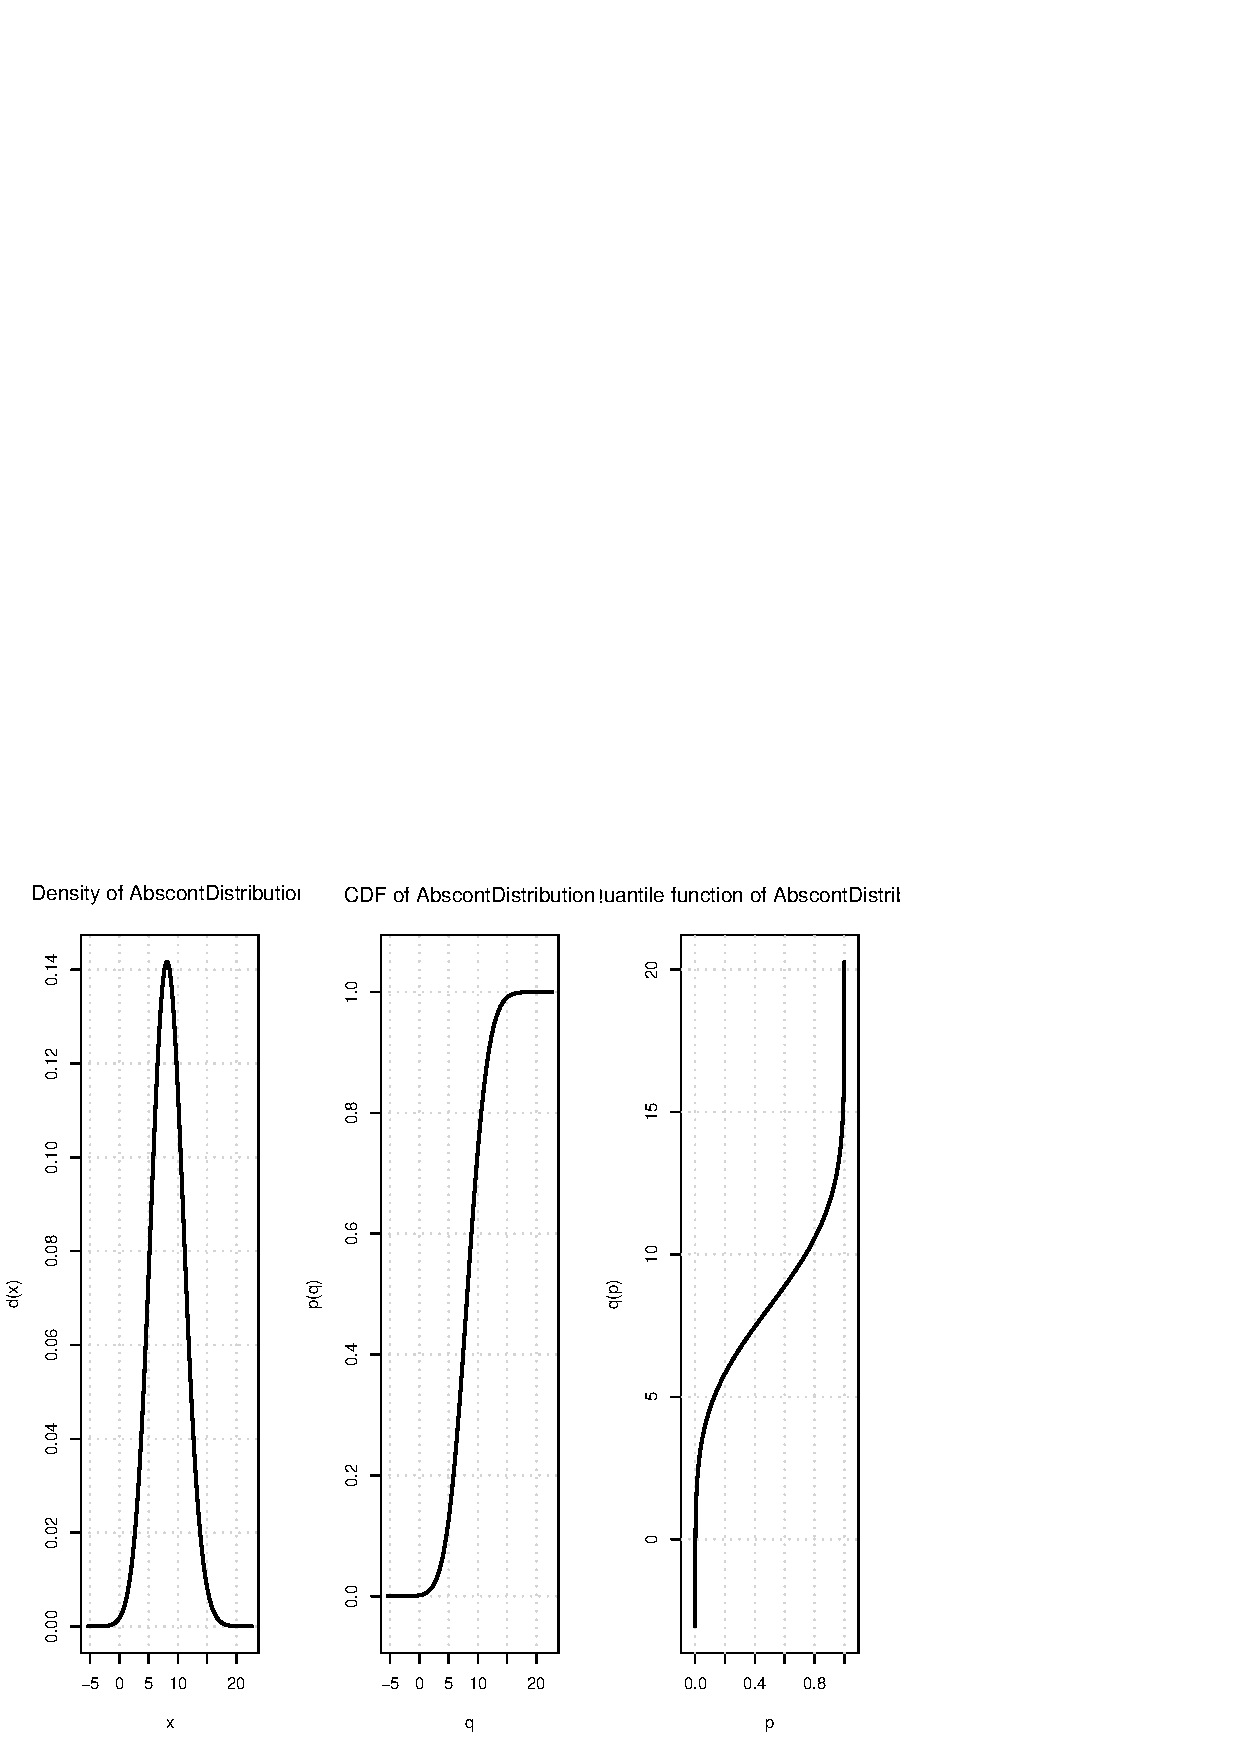
\includegraphics{newDistributions-exam1}
\par
\noindent{\bf Comment:}\\
Let \code{N} an object of class \code{"Norm"} with parameters  \code{mean=2},
\code{sd=1.3} and let \code{P}  an object of class \code{"Pois"} with parameter 
\code{lambda=1.2}. Assigning to \code{Z} the expression \code{2*N+3+P}, a 
new distribution object is generated ---of class \code{"AbscontDistribution"} in 
our case--- so that identifying \code{N}, \code{P}, \code{Z} with random 
variables distributed according to {\tt N}, {\tt P}, {\tt Z}, 
${\cal L}({\tt Z})={\cal L}(2*{\tt N}+3+{\tt P})$,  and writing \code{p(Z)(0.4)}  
we get $P(Z\leq 0.4)$, \code{ q(Z)(0.3)}  the $30\%$-quantile of {\tt Z},
and with \code{r(Z)(50)} we generate $50$ pseudo random numbers distributed 
according to {\tt Z}, while the \code{plot} command generates the above figure.\\

There a caveats to take care about; for details refer to the (larger) vignette
{\tt distr} in package \pkg{distrDoc}.
% -------------------------------------------------------------------------------
\section{Using generating functions}
% -------------------------------------------------------------------------------
If you want to generate a single distribution object (without any particular parameter)
generating functions are the method of choice:\\


Objects of classes \code{LatticeDistribution} resp.\ 
\code{DiscreteDistribution}, 
\code{AbscontDistribution},  may be generated using the generating functions
\code{LatticeDistribution()} resp.\ \code{DiscreteDistribution()}
resp.\ \code{AbscontDistribution()}; see also
the corresponding help.\\

E.g., to produce a discrete distribution with
support $(1,5,7,21)$ with corresponding probabilities $(0.1,0.1,0.6,0.2)$
we may write
\begin{Schunk}
\begin{Sinput}
> D <- DiscreteDistribution(supp = c(1,5,7,21), prob = c(0.1,0.1,0.6,0.2))
> D
\end{Sinput}
\begin{Soutput}
Distribution Object of Class: DiscreteDistribution
\end{Soutput}
\begin{Sinput}
> plot(D, panel.first = grid(), lwd = 2)
\end{Sinput}
\end{Schunk}
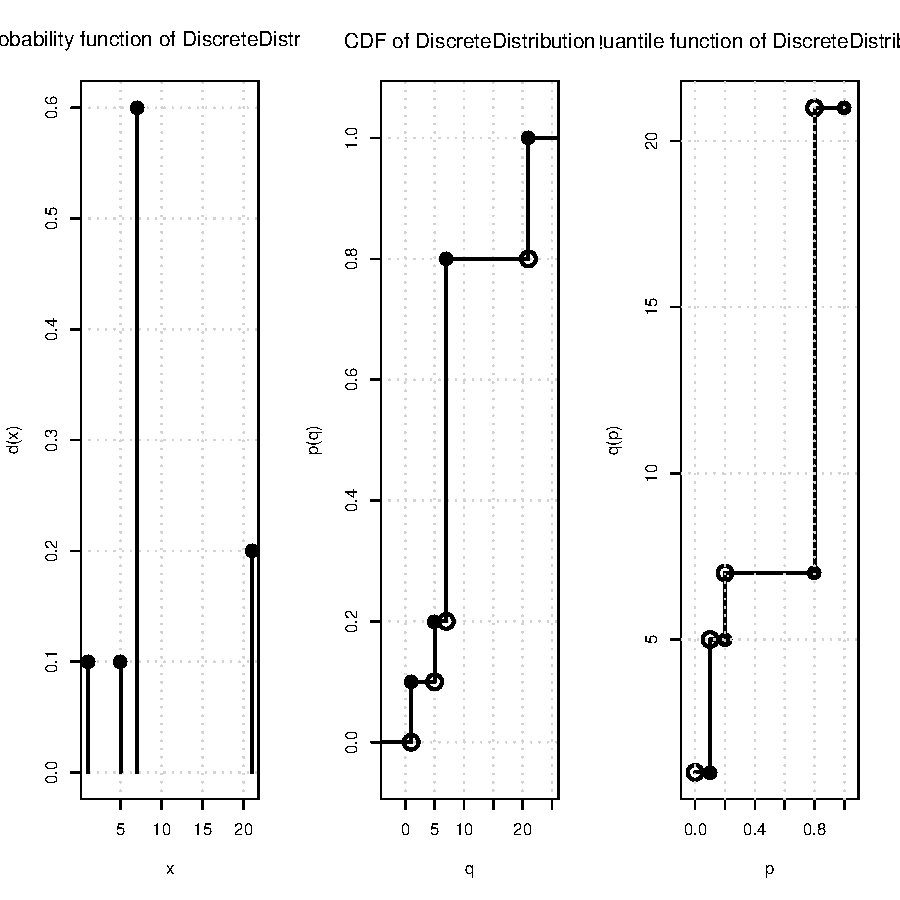
\includegraphics{newDistributions-DiscrDist}
%
\newline
and to generate an absolutely continuos distribution with density proportional
to $e^{-|x|^3}$, we write
\begin{Schunk}
\begin{Sinput}
> AC <- AbscontDistribution(d = function(x) exp(-abs(x)^3), withStand = TRUE)
> AC
\end{Sinput}
\begin{Soutput}
Distribution Object of Class: AbscontDistribution
\end{Soutput}
\begin{Sinput}
> plot(AC, panel.first = grid(), lwd = 2)
\end{Sinput}
\end{Schunk}
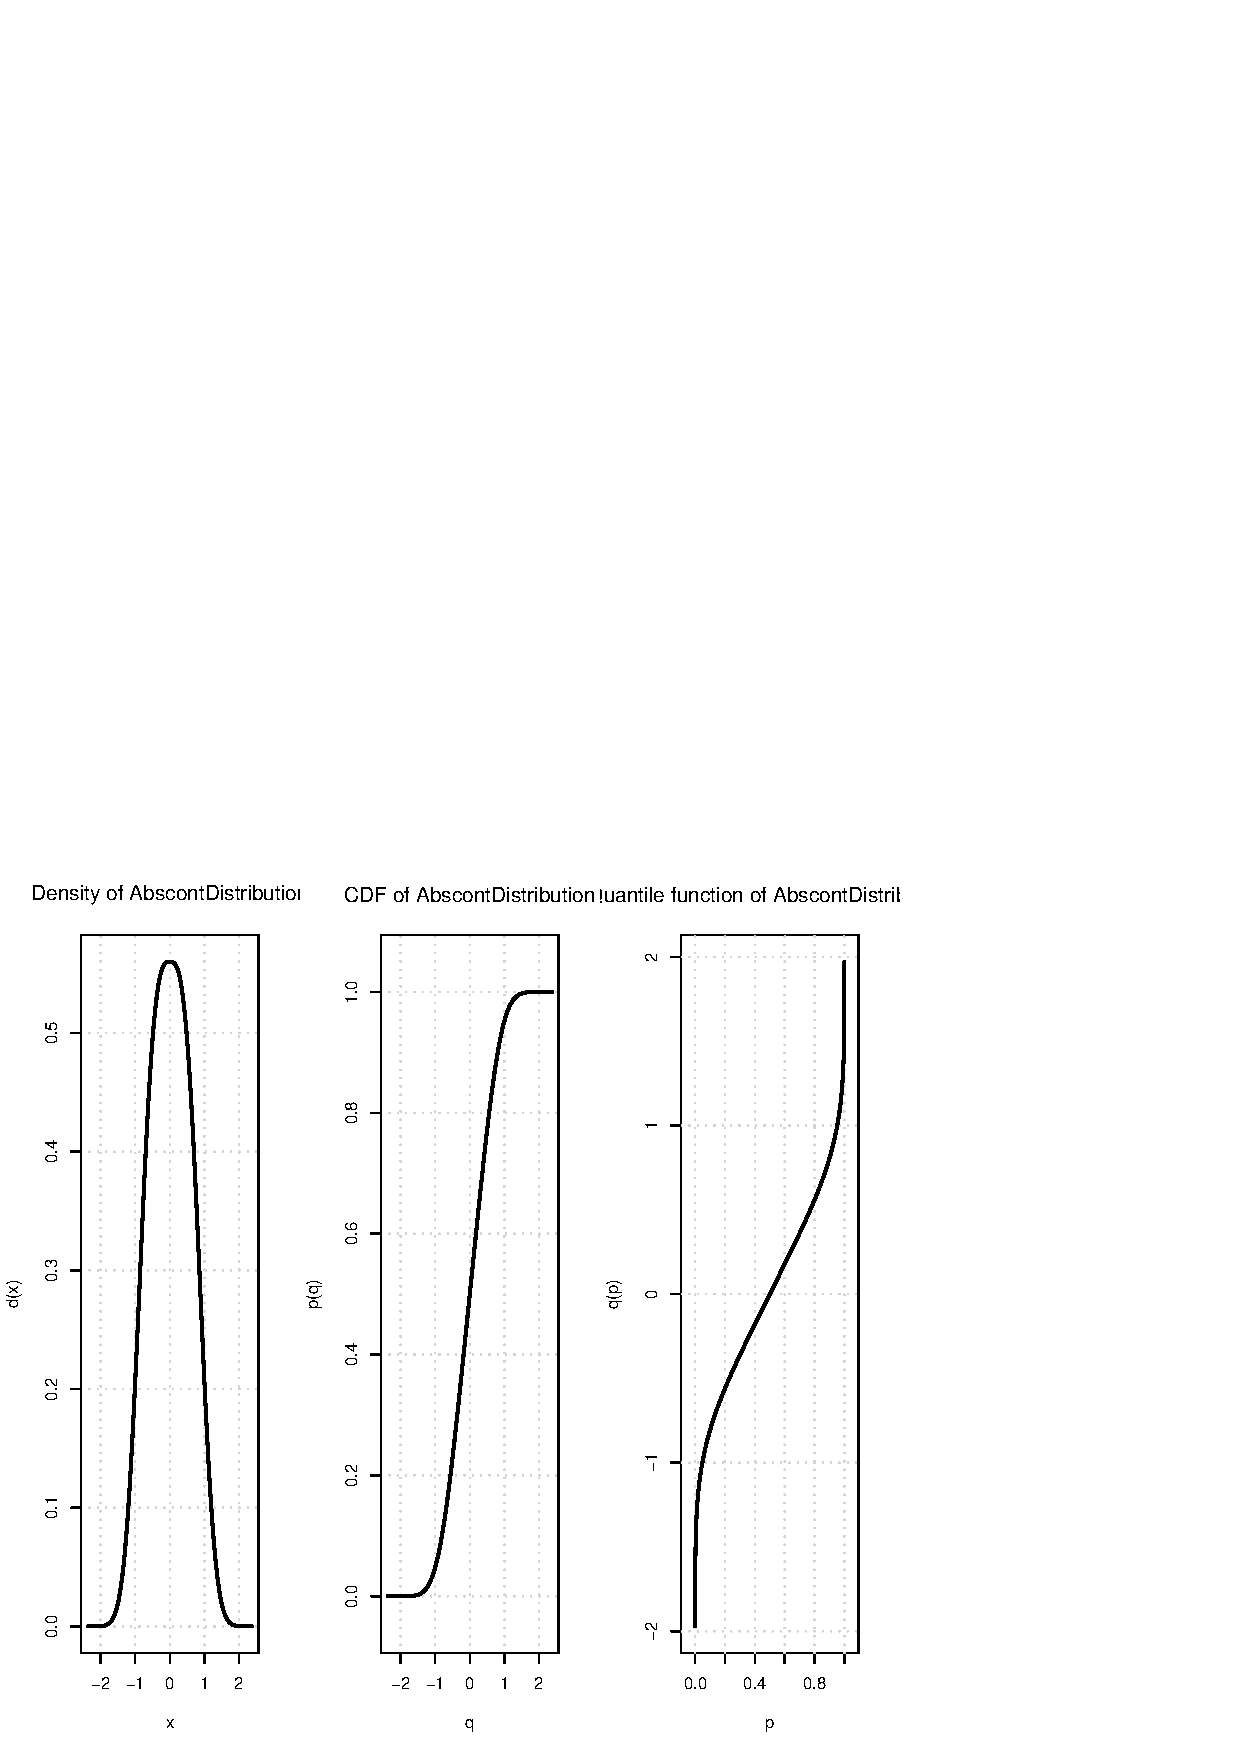
\includegraphics{newDistributions-AbscDist}
%
% -------------------------------------------------------------------------------
\section{Doing it from scratch}
% -------------------------------------------------------------------------------
If you would like to create new parametric distributions, using already 
implemented {\tt r}, {\tt d}, {\tt p}, and {\tt q} functions
(e.g.\ implementing additional distributions realized in another 
\href{http://cran.r-project.org}{\tt CRAN} package), 
you should probably envisage introducing new distribution {\tt S4} (sub-)classes
and hence better look at the implementation of some discrete and 
continuous parametric distribution classes in package \pkg{distr}.

\noindent{\small Hint: download the {\tt .tar.gz} file; extract it to some {\tt temp} 
folder; look at subdirectories {\tt R} and {\tt man}}\smallskip\\

The general procedure is as follows

\begin{enumerate}
\item introduce a  new subclass of  class \code{Parameter}
\item introduce a new subclass of  \code{LatticeDistribution}/%
\code{DiscreteDistribution} (if discrete)
 or of class \code{AbscontDistribution} (if continuous).
\item define accessor and replacement functions for the ``slots'' of the
parameter (e.g.\ \code{"size"} and \code{"prob"} in the binomial case), 
possibly with new generics
\item (possibly) define a validity function
\item define a generating function
\item if existing, define particular convolution methods or similar particular
methods for this new distribution class
\item create {\tt .Rd} files for the
\begin{itemize}
      \item parameter class
      \item distribution class
\end{itemize}
\item if analytic expressions are available, define particular \code{E}-, \code{var}-, 
\code{skewness}-, and \code{kurtosis}-methods
     and if so, also document\footnote{%
%
this is new, because so far, all \code{E}-, \code{var}-, 
\code{skewness}-, and \code{kurtosis}-methods for ``basic'' 
distributions are documented in the \pkg{distrEx} documentation to 
\code{E}, \code{var}, \ldots, but this would not be operational
any longer for new derived classes, possibly defined in other, new packages
%
     } the corresponding methods in
     the distribution class {\tt .Rd} file\\
\end{enumerate}
    
Let's go through the steps in the example case of the Binomial implementation
in packages \pkg{distr} and \pkg{distrEx}:

\begin{enumerate}
%
\item in \pkg{distr}, see source in \file{R/AllClasses.R},  
%
lines 180--189
%------------------------------------------------------------------------------%
\Rlstset
\begin{lstlisting}
## Class: BinomParameter
setClass("BinomParameter", 
          representation = representation(size = "numeric", prob = "numeric"), 
          prototype = prototype(size = 1, prob = 0.5, name = 
                      gettext("Parameter of a Binomial distribution")
                      ), 
          contains = "Parameter"
          )

#-
\end{lstlisting}
%------------------------------------------------------------------------------%
%%
\item in \pkg{distr}, see source in \file{R/AllClasses.R},  
%
lines 869--897
%------------------------------------------------------------------------------%
\Rlstset
\begin{lstlisting}
## Class: binomial distribution
setClass("Binom",
          prototype = prototype(
                      r = function(n){ rbinom(n, size = 1,prob = 0.5) },
                      d = function(x, log = FALSE){
                              dbinom(x, size = 1, prob = 0.5, log = log)
                                          },
                      p = function(q, lower.tail = TRUE, log.p = FALSE ){
                              pbinom(q, size = 1, prob = 0.5,
                                     lower.tail = lower.tail, log.p = log.p)
                                          },
                      q = function(p, lower.tail = TRUE, log.p = FALSE ){
                              qbinom(p, size = 1, prob = 0.5,
                                     lower.tail = lower.tail, log.p = log.p)
                                          },
                      img = new("Naturals"),
                      param = new("BinomParameter"),
                      support = 0:1,
                      lattice = new("Lattice",
                                pivot = 0, width = 1, Length = 2, name =
                                gettext(
                                  "lattice of a Binomial distribution"
                                       )
                                ),
                     .logExact = TRUE,
                     .lowerExact = TRUE
                      ),
          contains = "LatticeDistribution"
          )
\end{lstlisting}
%------------------------------------------------------------------------------%
%%
\item in \pkg{distr}, see source in \file{R/BinomialDistribution.R},  
%
lines 8--15, and
43--53
%------------------------------------------------------------------------------%
\Rlstset
\begin{lstlisting}
## Access Methods
setMethod("size", "BinomParameter", function(object) object@size)
setMethod("prob", "BinomParameter", function(object) object@prob)
## Replace Methods
setReplaceMethod("size", "BinomParameter", 
                  function(object, value){ object@size <- value; object})
setReplaceMethod("prob", "BinomParameter", 
                  function(object, value){ object@prob <- value; object})
\end{lstlisting}
%------------------------------------------------------------------------------%
%

%------------------------------------------------------------------------------%
\Rlstset
\begin{lstlisting}
## wrapped access methods
setMethod("prob", "Binom", function(object) prob(param(object)))
setMethod("size", "Binom", function(object) size(param(object)))
## wrapped replace methods
setMethod("prob<-", "Binom", 
           function(object, value) new("Binom", prob = value, 
                                        size = size(object)))
setMethod("size<-", "Binom", 
           function(object, value) new("Binom", prob = prob(object), 
                                        size = value))

\end{lstlisting}
%------------------------------------------------------------------------------%
%%
and \file{R/AllGenerics}, 
lines 143--146
%------------------------------------------------------------------------------%
\Rlstset
\begin{lstlisting}
if(!isGeneric("size")) 
   setGeneric("size", function(object) standardGeneric("size"))
if(!isGeneric("prob")) 
   setGeneric("prob", function(object) standardGeneric("prob"))
\end{lstlisting}
%------------------------------------------------------------------------------%
%%
\item in \pkg{distr}, see source in \file{R/BinomialDistribution.R},  
%
lines 18--32
%------------------------------------------------------------------------------%
\Rlstset
\begin{lstlisting}
setValidity("BinomParameter", function(object){
  if(length(prob(object)) != 1)
    stop("prob has to be a numeric of length 1")    
  if(prob(object) < 0)
    stop("prob has to be in [0,1]")
  if(prob(object) > 1)
    stop("prob has to be in [0,1]")
  if(length(size(object)) != 1)
    stop("size has to be a numeric of length 1")    
  if(size(object) < 1)
    stop("size has to be a natural greater than 0")
  if(!identical(floor(size(object)), size(object)))
    stop("size has to be a natural greater than 0")    
  else return(TRUE)
})
\end{lstlisting}
%------------------------------------------------------------------------------%
%%
\item in \pkg{distr}, see source in \file{R/BinomialDistribution.R},  
%
line 41
%------------------------------------------------------------------------------%
\Rlstset
\begin{lstlisting}
Binom <- function(size = 1,prob = 0.5) new("Binom", size = size, prob = prob)
\end{lstlisting}
%------------------------------------------------------------------------------%
%%
\item in \pkg{distr}, see source in \file{R/BinomialDistribution.R},  
%
lines 54--68
%------------------------------------------------------------------------------%
\Rlstset
\begin{lstlisting}
## Convolution for two binomial distributions Bin(n1,p1) and Bin(n2,p2)
## Distinguish cases 
## p1 == p2 und p1 != p2


setMethod("+", c("Binom","Binom"),
          function(e1,e2){
            newsize <- size(e1) + size(e2)
            
            if(isTRUE(all.equal(prob(e1),prob(e2))))    
               return(new("Binom", prob = prob(e1), size = newsize, 
                          .withArith = TRUE))
            
            return(as(e1, "LatticeDistribution") + e2)
          })
\end{lstlisting}
%------------------------------------------------------------------------------%
%%
\item in \pkg{distr}, see sources in
%
\begin{itemize}
%
\item\file{man/BinomParameter-class.Rd}
%
%------------------------------------------------------------------------------%
\begin{lstlisting}[style=Rdstyle]
\name{BinomParameter-class} 
\docType{class}
\alias{BinomParameter-class}
\alias{initialize,BinomParameter-method}

\title{Class "BinomParameter"}
\description{ The parameter of a binomial distribution, used by Binom-class}
\section{Objects from the Class}{
Objects can be created by calls of the form 
      \code{new("BinomParameter", prob, size)}.
Usually an object of this class is not needed on its own, it is generated 
automatically when an object of the class Binom
is instantiated. 
}
\section{Slots}{
  \describe{
    \item{\code{prob}:}{Object of class \code{"numeric"}: 
          the probability of a binomial distribution }
    \item{\code{size}:}{Object of class \code{"numeric"}: 
          the size of a binomial distribution }
    \item{\code{name}:}{Object of class \code{"character"}: 
          a name / comment for the parameters }
  }
}
\section{Extends}{
Class \code{"Parameter"}, directly.
}
\section{Methods}{
  \describe{
    \item{initialize}{\code{signature(.Object = "BinomParameter")}: 
          initialize method }
    \item{prob}{\code{signature(object = "BinomParameter")}: returns the slot 
          \code{prob} of the parameter of the distribution }
    \item{prob<-}{\code{signature(object = "BinomParameter")}: modifies the slot 
          \code{prob} of the parameter of the distribution }
    \item{size}{\code{signature(object = "BinomParameter")}: returns the slot 
          \code{size} of the parameter of the distribution }
    \item{size<-}{\code{signature(object = "BinomParameter")}: modifies the slot 
          \code{size} of the parameter of the distribution}
  }
}

\author{
  Thomas Stabla \email{statho3@web.de},\cr 
  Florian Camphausen \email{fcampi@gmx.de},\cr
  Peter Ruckdeschel \email{Peter.Ruckdeschel@itwm.fraunhofer.de},\cr 
  Matthias Kohl \email{Matthias.Kohl@stamats.de}
  }


\seealso{
\code{\link{Binom-class}}
\code{\link{Parameter-class}}
}

\examples{
\end{lstlisting}\vspace{-2ex}
%------------------------------------------------------------------------------%
\begin{lstlisting}[style=Rstyle,basicstyle = \scriptsize\color{Rcolor}, xleftmargin = 2em]
W <- new("BinomParameter",prob=0.5,size=1)
size(W) # size of this distribution is 1.
size(W) <- 2 # size of this distribution is now 2.
\end{lstlisting}\vspace{-3ex}
%------------------------------------------------------------------------------%
\begin{lstlisting}[style=Rdstyle]
}
\keyword{distribution}
\concept{parameter}
\concept{Binomial distribution}
\concept{S4 parameter class}
\end{lstlisting}
%------------------------------------------------------------------------------%
%%
\item\file{man/Binom-class.Rd}
%------------------------------------------------------------------------------%
\begin{lstlisting}[style=Rdstyle]
\name{Binom-class} 
\docType{class}
\alias{Binom-class}
\alias{Binom}
\alias{initialize,Binom-method}

\title{Class "Binom" }
\description{The binomial distribution with \code{size} \eqn{= n}, by default 
  \eqn{=1}, and
  \code{prob} \eqn{= p}, by default \eqn{=0.5}, has density
  \deqn{p(x) = {n \choose x} {p}^{x} {(1-p)}^{n-x}}{
    p(x) = choose(n,x) p^x (1-p)^(n-x)}
  for \eqn{x = 0, \ldots, n}.

  C.f.\code{\link[stats:Binomial]{rbinom}}
}
\section{Objects from the Class}{
Objects can be created by calls of the form \code{Binom(prob, size)}.
This object is a binomial distribution. 
}
\section{Slots}{
  \describe{
    \item{\code{img}:}{Object of class \code{"Naturals"}: The space of the 
     image of this distribution has got dimension 1 and the 
     name "Natural Space". }
    \item{\code{param}:}{Object of class \code{"BinomParameter"}: the parameter 
          of this distribution (\code{prob}, \code{size}), declared at its 
          instantiation }
    \item{\code{r}:}{Object of class \code{"function"}: generates random 
          numbers (calls function \code{rbinom}) }
    \item{\code{d}:}{Object of class \code{"function"}: density function (calls 
          function \code{dbinom}) }
    \item{\code{p}:}{Object of class \code{"function"}: cumulative function 
          (calls function \code{pbinom}) }
    \item{\code{q}:}{Object of class \code{"function"}: inverse of the 
           cumulative function (calls function \code{qbinom}).
    The quantile is defined as the smallest value x such that F(x) >= p, where 
            F is the cumulative function. }
    \item{\code{support}:}{Object of class \code{"numeric"}: a (sorted) 
            vector containing the support of the discrete density function}
    \item{\code{.withArith}:}{logical: used internally to issue warnings as to interpretation of arithmetics}
    \item{\code{.withSim}:}{logical: used internally to issue warnings as to accuracy}
    \item{\code{.logExact}:}{logical: used internally to flag the case where there are explicit formulae for the
                              log version of density, cdf, and quantile function}
    \item{\code{.lowerExact}:}{logical: used internally to flag the case where there are explicit formulae for the
                              lower tail version of cdf and quantile function}
  }
}
\section{Extends}{
Class \code{"DiscreteDistribution"}, directly.\cr
Class \code{"UnivariateDistribution"}, by class \code{"DiscreteDistribution"}.\cr
Class \code{"Distribution"}, by class \code{"DiscreteDistribution"}.
}
\section{Methods}{
  \describe{
    \item{+}{\code{signature(e1 = "Binom", e2 = "Binom")}: For two binomial 
             distributions with equal probabilities the exact convolution 
             formula is implemented thereby improving the general numerical 
             accuracy.}
    \item{initialize}{\code{signature(.Object = "Binom")}: initialize method }
    \item{prob}{\code{signature(object = "Binom")}: returns the slot \code{prob} 
             of the parameter of the distribution }
    \item{prob<-}{\code{signature(object = "Binom")}: modifies the slot 
             \code{prob} of the parameter of the distribution }
    \item{size}{\code{signature(object = "Binom")}: returns the slot \code{size} 
             of the parameter of the distribution }
    \item{size<-}{\code{signature(object = "Binom")}: modifies the slot 
             \code{size} of the parameter of the distribution }
  }
}


\author{
  Thomas Stabla \email{statho3@web.de},\cr 
  Florian Camphausen \email{fcampi@gmx.de},\cr
  Peter Ruckdeschel \email{Peter.Ruckdeschel@itwm.fraunhofer.de},\cr 
  Matthias Kohl \email{Matthias.Kohl@stamats.de}
  }


\seealso{
\code{\link{BinomParameter-class}}
\code{\link{DiscreteDistribution-class}}
\code{\link{Naturals-class}}
\code{\link[stats:Binomial]{rbinom}}
}
\examples{
\end{lstlisting}\vspace{-2ex}
%------------------------------------------------------------------------------%
\begin{lstlisting}[style=Rstyle,basicstyle = \scriptsize\color{Rcolor}, xleftmargin = 2em]
B <- Binom(prob=0.5,size=1) # B is a binomial distribution with prob=0.5 and size=1.
r(B)(1) # # one random number generated from this distribution, e.g. 1
d(B)(1) # Density of this distribution is  0.5 for x=1.
p(B)(0.4) # Probability that x<0.4 is 0.5.
q(B)(.1) # x=0 is the smallest value x such that p(B)(x)>=0.1.
size(B) # size of this distribution is 1.
size(B) <- 2 # size of this distribution is now 2.
C <- Binom(prob = 0.5, size = 1) # C is a binomial distribution with prob=0.5 and size=1.
D <- Binom(prob = 0.6, size = 1) # D is a binomial distribution with prob=0.6 and size=1.
E <- B + C # E is a binomial distribution with prob=0.5 and size=3.
F <- B + D # F is an object of class LatticeDistribution.
G <- B + as(D,"DiscreteDistribution") ## DiscreteDistribution
\end{lstlisting}\vspace{-3ex}
%------------------------------------------------------------------------------%
\begin{lstlisting}[style=Rdstyle]
}
\keyword{distribution}
\concept{discrete distribution}
\concept{lattice distribution}
\concept{Binomial family}
\concept{Binomial distribution}
\concept{S4 distribution class}
\concept{generating function}
\end{lstlisting}
%------------------------------------------------------------------------------%
%%
\item {\footnotesize you could have: \file{man/Binom.Rd}
      for the generating function; in the Binomial case, documentation is in
      \file{Binom-class.Rd}; but in case of the Gumbel distribution,
      in package \pkg{distrEx}, there is such an extra {\tt .Rd} file}
%
\end{itemize}
%
\item in \pkg{distrEx}, see sources in
%
